\section{Network Construction and Operation}

This work mainly follows the temporal neuron as defined in \cite{TNN}. As such,
this section presents an overview of the network construction process and
the individual (hyper)parameters of a constructed network.

\begin{figure}[h]
    \centering
    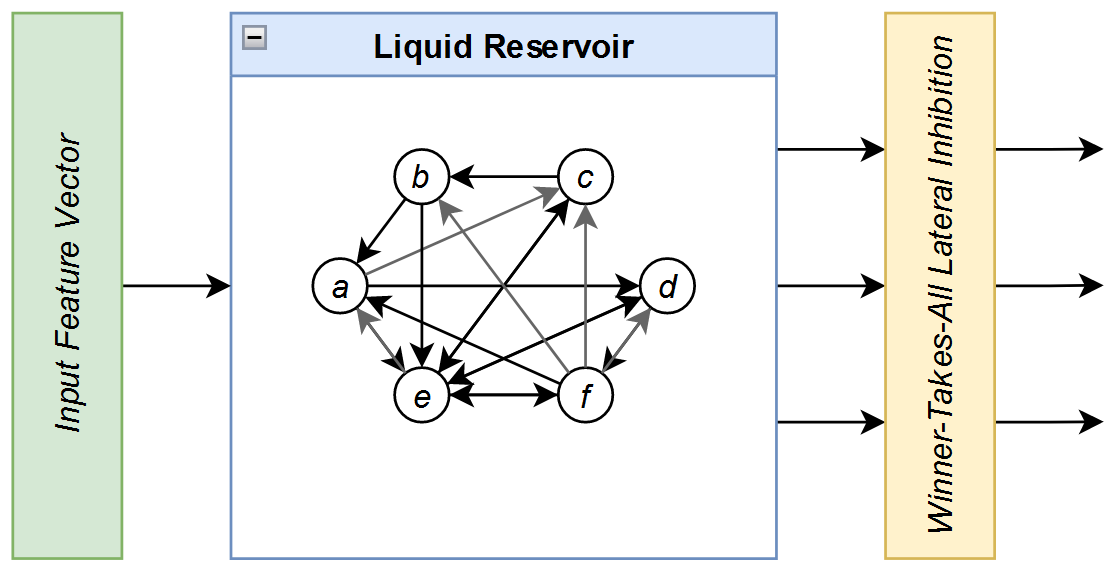
\includegraphics[scale=0.25]{tlsm_diagram.png}
    \caption{Diagram of a temporal liquid state machine (TLSM).}
    \label{fig:tlsm_diagram}
\end{figure}

The overall temporal liquid state machine, as depicted in figure
\ref{fig:tlsm_diagram}, consists of an input feature vector, a reservoir, and an
output column. This entire structure (composed of three parts) implements an
unsupervised online learning algorithm, and is heavily parameterized.

\subsection{Input Feature Vector}

The input feature vector is a one-dimensional time-encoded vector of the input
values discretized and normalized in some arbitrary capacity. As temporal
neurons are intended to be good-for-hardware models, they are simply integral
in type (as per \cite{TNN}). As such, the input vector is also integral in type.

The inputs are encoded as time spikes, where a 'higher' value corresponds to a
quicker spike (with a lower 'entry time'). These spikes notably do not have any
magnitude associated with them, and are simply an impulse function on the line.

The choice of input encoding is arbitrary, and is focused on more in section
\ref{sec:Problem-Specific Analysis} for each problem. However, some notable
features of 'good' encoding schemes for biologically inspired neural networks
are discussed in \cite{Encoding}. In particular, the overlapping of contextual
information is a key feature of good encoding schemes - 'Proximal' patterns can
be encoded in a way that allows for the network to learn similarities between
input patterns.

\subsection{Network Configuration}

The reservoir contains a series of neurons, the number of which is a
hyperparameter to the network. Each neuron within the reservoir is connected to
other neurons in some particular way. This connectivity is, itself, another
hyperparameter of the network. As such, the reservoir (upon initialization)
takes in a 'seed matrix' $W_0$. For a TLSM of size $n$, this matrix is of size
$n\times n$. The seed matrix forms an adjacency matrix for the reservoir,
indicating its connectivity.

There are two particular features regarding the network indicated by the seed
matrix. For one, the seed matrix may be asymmetric. This makes the output
network a directed graph. Secondly, the seed matrix may be sparse and is not
necessarily fully connected. The construction of the seed matrix may be done
using one of many random graph algorithms, such as the Erdos-Renyi model or the
Barabasi-Albert model. We leave this choice as a hyperparameter as well, opting
to implement several different connectivity models to test their performance
individually for each problem.

\subsection{Neuron Activation Functions}

Lorem ipsum

\subsection{Network Training}

Lorem ipsum